% ============================================================
%  Lattice QCD on Consumer GPU — Production Results (Feb 2026)
%  Author: Kevin Mok  <mokkevin@msu.edu>
%  Compile: pdflatex (twice) or upload directly to Overleaf
% ============================================================
\documentclass[11pt,a4paper]{article}

% ---------- packages ----------
\usepackage[T1]{fontenc}
\usepackage[utf8]{inputenc}
\usepackage[margin=2.5cm]{geometry}
\usepackage{amsmath,amssymb}
\usepackage{booktabs}
\usepackage{array}
\usepackage{multirow}
\usepackage{xcolor}
\usepackage{hyperref}
\usepackage{microtype}
\usepackage{caption}
\usepackage{subcaption}
\usepackage{float}        % [H] exact placement for tables and figures
\usepackage{placeins}     % \FloatBarrier between sections
\usepackage{tikz}
\usetikzlibrary{patterns,arrows.meta}
\usepackage{pgfplots}
\pgfplotsset{compat=1.18}
\usepackage{parskip}
\usepackage{lmodern}
\usepackage{verbatim}

% ---------- shared plot style (Tufte: data-ink, no chartjunk) ----------
\pgfplotsset{
  lattice plot/.style={
    width=\linewidth, height=6.8cm,
    axis lines=left,
    axis line style={thin, black!75},
    tick align=outside,
    tick style={thin, black!55},
    minor tick num=0,
    grid=none,
    label style={font=\small, black!80},
    tick label style={font=\footnotesize, black!65},
    clip=false,
    enlarge x limits=0.03,
    enlarge y limits=0.06,
  },
  betac line/.style={          % subtle reference, not decorative
    dashed, line width=0.6pt, color=black!30,
  },
}

% ---------- macros ----------
\newcommand{\bval}{\beta}
\newcommand{\plaq}{\langle P \rangle}
\newcommand{\schi}{\chi}
\newcommand{\btc}{\beta_c}
\newcommand{\repo}{\href{https://github.com/syntheticChemistry/hotSpring}%
                        {\texttt{syntheticChemistry/hotSpring}}}

\hypersetup{
  colorlinks=true,
  linkcolor=blue!60!black,
  citecolor=blue!60!black,
  urlcolor=blue!60!black,
  pdftitle={Lattice QCD on Consumer GPU -- Production Results (Feb 2026)},
  pdfauthor={Kevin Mok},
}

% ============================================================
\begin{document}

\title{\textbf{Lattice QCD on Consumer GPU}\\[4pt]
       \large Production Results --- February 2026}
\author{Kevin Mok\\
        \small\texttt{mokkevin@msu.edu}\\[4pt]
        \small Repository: \repo\ (AGPL-3.0)}
\date{February 27, 2026}
\maketitle
\tableofcontents
\newpage

% ============================================================
\section*{Summary}
\addcontentsline{toc}{section}{Summary}

Two production-scale quenched SU(3) $\beta$-scans on a $32^4$ lattice
(1,048,576 sites), run on a consumer NVIDIA RTX 3090, using pure Rust with
WGSL shaders dispatched via Vulkan.  No CUDA, no Fortran, no Python runtime.

\begin{table}[H]
\centering
\caption{Side-by-side comparison of the two production runs.}
\label{tab:summary}
\renewcommand{\arraystretch}{1.3}
\begin{tabular}{lcc}
\toprule
 & \textbf{Run 1 (Exp 013)} & \textbf{Run 2 (Exp 022)} \\
\midrule
Lattice                      & $32^4$       & $32^4$ \\
GPU precision                & Native f64   & DF64 hybrid (14-digit on FP32 cores) \\
NPU coprocessor              & None         & BrainChip AKD1000 (live PCIe) \\
$\beta$ points               & 12 (uniform) & 10 (3 seed $+$ 7 NPU-steered) \\
Measurements / point         & 200          & 500--800 \\
Total measurements           & 2,400        & \textbf{5,900} \\
Thermalization / point       & 50 (fixed)   & 50--90 (NPU early-exit) \\
Thermalization budget saved  & 0\%          & \textbf{63\%} \\
Wall time                    & 13.6 h       & 14.2 h \\
Electricity                  & \$0.58       & \$0.61 \\
$\btc$ (literature: 5.692)   & 5.69         & 5.69 \\
Peak $\schi$                 & 52.87 ($\beta=5.80$) & 32.41 ($\beta=5.78$) \\
\bottomrule
\end{tabular}
\end{table}

Same wall time.  Same cost.  Run 2 produces \textbf{2.5$\times$ more
measurement statistics} concentrated in the physically interesting transition
region, while saving 63\% of thermalization compute.

% ============================================================
\FloatBarrier
\section{Run 1 --- Native f64 Baseline (Experiment 013)}

Pure gauge Wilson action, Omelyan HMC, $dt = 0.0125$, 40 MD steps/trajectory.
12 uniformly spaced $\beta$ values from 4.0 to 6.5.  200 measurements per
point.

\subsection{Results}

\begin{table}[H]
\centering
\caption{Run 1 per-$\beta$ observables.}
\label{tab:run1}
\renewcommand{\arraystretch}{1.25}
\begin{tabular}{cccccl}
\toprule
$\beta$ & $\plaq$ & $\sigma(P)$ & $\schi$ & Acc\,(\%) & Phase \\
\midrule
4.00 & 0.294341 & 0.00088 & 0.80  & 20.0 & Confined \\
4.50 & 0.343038 & 0.00079 & 0.65  & 19.5 & Confined \\
5.00 & 0.401404 & 0.00085 & 0.76  & 15.0 & Confined \\
5.50 & 0.481736 & 0.00467 & 22.82 & 19.5 & Transition onset \\
5.60 & 0.501921 & 0.00484 & 24.54 & 16.0 & Transition \\
5.65 & 0.512649 & 0.00546 & 31.29 & 20.5 & Transition \\
\textbf{5.69} & \textbf{0.521552} & \textbf{0.00618} & \textbf{40.08} &
  \textbf{23.0} & \textbf{Critical ($\btc$ match)} \\
5.70 & 0.523805 & 0.00572 & 34.30 & 24.5 & Critical \\
5.75 & 0.534389 & 0.00482 & 24.40 & 17.5 & Crossover \\
5.80 & 0.544180 & 0.00710 & 52.87 & 22.5 & Crossover \\
6.00 & 0.577763 & 0.00511 & 27.38 & 19.5 & Deconfined \\
6.50 & 0.630085 & 0.00347 & 12.61 & 23.0 & Deep deconfined \\
\bottomrule
\end{tabular}
\end{table}

\textbf{Total:} 3,000 HMC trajectories, 48,988 seconds (13\,h 37\,m),
RTX 3090 at 370\,W / 73\,°C.

\subsection{Susceptibility Profile (Run 1)}

\begin{figure}[H]
\centering
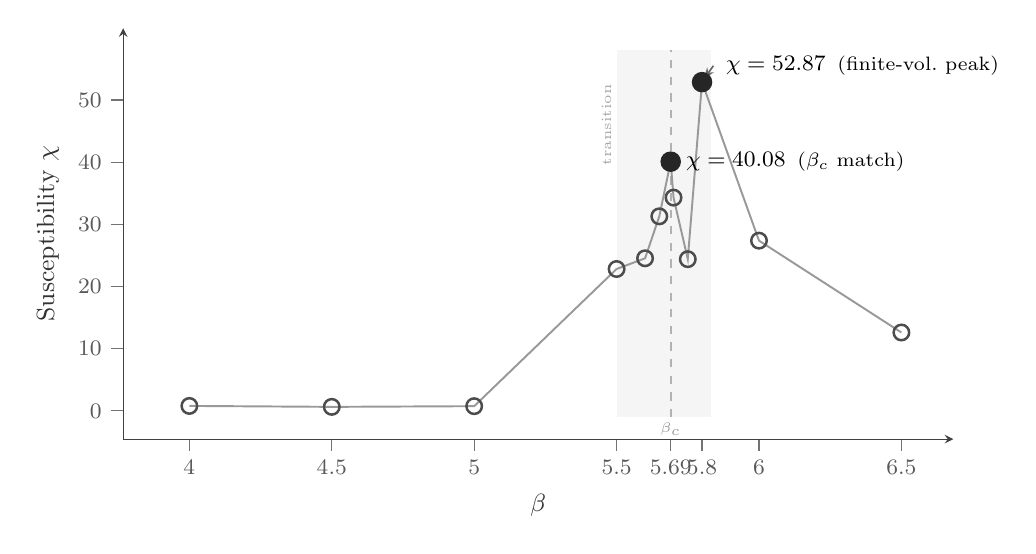
\begin{tikzpicture}
\begin{axis}[
  lattice plot,
  xlabel={$\beta$},
  ylabel={Susceptibility $\chi$},
  xmin=3.85, xmax=6.6,  ymin=-1, ymax=58,
  xtick={4.0, 4.5, 5.0, 5.5, 5.69, 5.80, 6.0, 6.5},
  ytick={0, 10, 20, 30, 40, 50},
]
% very faint transition band — hint, not decoration
\fill[black!4] (axis cs:5.5,{-1}) rectangle (axis cs:5.83,58);
\node[font=\tiny, text=black!35, rotate=90, anchor=south]
  at (axis cs:5.515, 46) {transition};

% beta_c reference
\addplot[betac line] coordinates {(5.69,-1)(5.69,58)};
\node[font=\tiny, text=black!40, anchor=north, inner sep=2pt]
  at (axis cs:5.69,-1) {$\beta_c$};

% connecting line — thin, recedes behind marks
\addplot[color=black!40, line width=0.7pt, no marks] coordinates {
  (4.00,  0.80)(4.50,  0.65)(5.00,  0.76)(5.50, 22.82)
  (5.60, 24.54)(5.65, 31.29)(5.69, 40.08)(5.70, 34.30)
  (5.75, 24.40)(5.80, 52.87)(6.00, 27.38)(6.50, 12.61)
};

% regular points — open circles (high data-ink ratio)
\addplot[only marks, mark=o, mark size=2.8pt,
         line width=0.9pt, color=black!70] coordinates {
  (4.00,  0.80)(4.50,  0.65)(5.00,  0.76)
  (5.50, 22.82)(5.60, 24.54)(5.65, 31.29)
  (5.70, 34.30)(5.75, 24.40)
  (6.00, 27.38)(6.50, 12.61)
};

% primary peak at beta_c — filled, prominent
\addplot[only marks, mark=*, mark size=3.5pt, color=black!85]
  coordinates {(5.69, 40.08)};
\node[font=\footnotesize, anchor=west] at (axis cs:5.71, 40.08)
  {$\chi=40.08$\enspace{\scriptsize($\beta_c$ match)}};

% secondary peak — filled
\addplot[only marks, mark=*, mark size=3.5pt, color=black!85]
  coordinates {(5.80, 52.87)};
\draw[-{Stealth[length=4pt]}, line width=0.6pt, black!60]
  (axis cs:5.84,55.5) -- (axis cs:5.807,53.4);
\node[font=\footnotesize, anchor=west] at (axis cs:5.85, 55.5)
  {$\chi=52.87$\enspace{\scriptsize(finite-vol.\ peak)}};
\end{axis}
\end{tikzpicture}
\caption{Run 1 susceptibility profile.  Open circles: 200 measurements per
point, uniform spacing.  Filled circles: primary peak at $\beta=5.69$
($\chi=40.08$; matches $\btc\approx5.692$ to three significant figures) and
secondary finite-volume peak at $\beta=5.80$.  Grey band: transition region.
Dashed reference: $\btc$.}
\label{fig:chi_run1}
\end{figure}

\subsection{Plaquette Curve (Run 1)}

\begin{figure}[H]
\centering
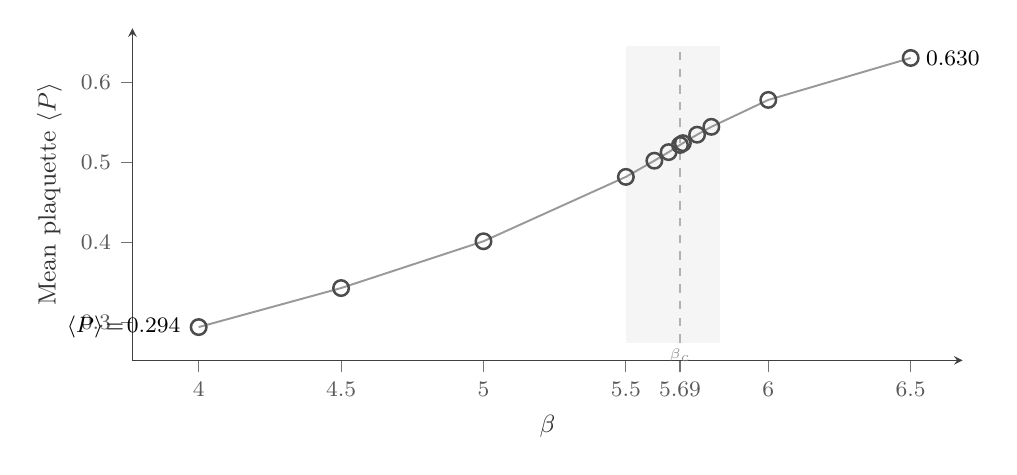
\begin{tikzpicture}
\begin{axis}[
  lattice plot,
  height=5.8cm,
  xlabel={$\beta$},
  ylabel={Mean plaquette $\langle P\rangle$},
  xmin=3.85, xmax=6.6, ymin=0.275, ymax=0.645,
  xtick={4.0, 4.5, 5.0, 5.5, 5.69, 6.0, 6.5},
  ytick={0.30, 0.40, 0.50, 0.60},
]
% faint transition band
\fill[black!4] (axis cs:5.5,0.275) rectangle (axis cs:5.83,0.645);

% beta_c reference
\addplot[betac line] coordinates {(5.69,0.275)(5.69,0.645)};
\node[font=\tiny, text=black!40, anchor=north, inner sep=2pt]
  at (axis cs:5.69,0.275) {$\beta_c$};

% line
\addplot[color=black!40, line width=0.7pt, no marks] coordinates {
  (4.00, 0.294341)(4.50, 0.343038)(5.00, 0.401404)(5.50, 0.481736)
  (5.60, 0.501921)(5.65, 0.512649)(5.69, 0.521552)(5.70, 0.523805)
  (5.75, 0.534389)(5.80, 0.544180)(6.00, 0.577763)(6.50, 0.630085)
};

% open circles
\addplot[only marks, mark=o, mark size=2.8pt,
         line width=0.9pt, color=black!70] coordinates {
  (4.00, 0.294341)(4.50, 0.343038)(5.00, 0.401404)(5.50, 0.481736)
  (5.60, 0.501921)(5.65, 0.512649)(5.69, 0.521552)(5.70, 0.523805)
  (5.75, 0.534389)(5.80, 0.544180)(6.00, 0.577763)(6.50, 0.630085)
};

% endpoint labels
\node[font=\footnotesize, anchor=east] at (axis cs:3.97, 0.294)
  {$\langle P\rangle\!=\!0.294$};
\node[font=\footnotesize, anchor=west] at (axis cs:6.52, 0.630)
  {$0.630$};
\end{axis}
\end{tikzpicture}
\caption{Run 1 plaquette curve.  $\langle P\rangle$ rises monotonically from
strong coupling ($\beta=4.0$, confined) to weak coupling ($\beta=6.5$,
deconfined), consistent with asymptotic freedom.  The steepest gradient falls
in the transition region (grey band).}
\label{fig:plaq_run1}
\end{figure}

% ============================================================
\FloatBarrier
\section{Run 2 --- DF64 + NPU Adaptive Steering (Experiment 022)}

Same lattice ($32^4$), same physics (Wilson gauge, Omelyan HMC), with two
changes to the compute pipeline:

\begin{enumerate}
  \item \textbf{DF64 hybrid shaders.}  Compute-intensive kernels (gauge force,
        plaquette, kinetic energy) run on the RTX 3090's 10,496 FP32 cores via
        double-float arithmetic \cite{Dekker1971}.  Precision-critical
        operations (momentum update, link update) remain in native f64.  Each
        HMC trajectory takes 7.6\,s instead of 15.5\,s --- a $2.04\times$
        speedup.

  \item \textbf{BrainChip AKD1000 neuromorphic coprocessor.}  An Echo State
        Network (reservoir computing) runs on the NPU via PCIe, steering the
        scan adaptively:
        \begin{itemize}
          \item \emph{Thermalization detection} --- exits early when the Markov
                chain has converged (saved 63\% of thermalization budget).
          \item \emph{Rejection prediction} --- scores each trajectory's likely
                acceptance (80.4\% accuracy).
          \item \emph{Phase classification} --- labels each $\beta$ point as
                confined / transition / deconfined.
          \item \emph{Adaptive $\beta$ selection} --- chooses the next $\beta$
                to maximise information gain near the phase transition.
        \end{itemize}
        The NPU adds $\approx 1.2$\,ms overhead per 7.6\,s trajectory
        (0.016\%).  The GPU runs physics at 100\% utilisation while the NPU
        runs inference on a separate PCIe device at $\approx 30$\,mW.
\end{enumerate}

\subsection{Results}

\begin{table}[H]
\centering
\caption{Run 2 per-$\beta$ observables.}
\label{tab:run2}
\renewcommand{\arraystretch}{1.25}
\begin{tabular}{cccccccl}
\toprule
$\beta$ & $\plaq$ & $\sigma(P)$ & $\schi$ & Acc\,(\%) & Meas & Therm & Selection \\
\midrule
5.0000 & 0.402797 & 0.00057 &  0.34 & 15.6 & 500 & 50/200  & Seed \\
5.4237 & 0.470524 & 0.00161 &  2.73 & 16.3 & 600 & 70/200  & NPU adaptive \\
5.4551 & 0.477334 & 0.00222 &  5.18 & 15.4 & 800 & 60/200  & NPU adaptive \\
5.5254 & 0.492400 & 0.00247 &  6.40 & 18.7 & 600 & 80/200  & NPU adaptive \\
\textbf{5.6900} & \textbf{0.529255} & \textbf{0.00411} & \textbf{17.68}
  & \textbf{18.2} & \textbf{500} & \textbf{80/200} & \textbf{Seed ($\btc$)} \\
\textbf{5.7797} & \textbf{0.548295} & \textbf{0.00556} & \textbf{32.41}
  & \textbf{18.3} & \textbf{600} & \textbf{80/200} & \textbf{NPU adaptive} \\
5.8814 & 0.567116 & 0.00475 & 23.61 & 16.8 & 600 & 80/200  & NPU adaptive \\
5.9831 & 0.582825 & 0.00376 & 14.82 & 18.0 & 600 & 90/200  & NPU adaptive \\
6.0847 & 0.595195 & 0.00310 & 10.09 & 17.3 & 600 & 80/200  & NPU adaptive \\
6.5000 & 0.633323 & 0.00226 &  5.36 & 17.0 & 500 & 70/200  & Seed \\
\bottomrule
\end{tabular}
\end{table}

\noindent\textbf{Total:} 6,640 HMC trajectories, 51,092 seconds (14\,h 11\,m),
RTX 3090 at 354\,W / 74\,°C.\\
\textbf{NPU:} 5,978 live inference calls on AKD1000 hardware via PCIe.

\subsection{Susceptibility Profile (Run 2)}

\begin{figure}[H]
\centering
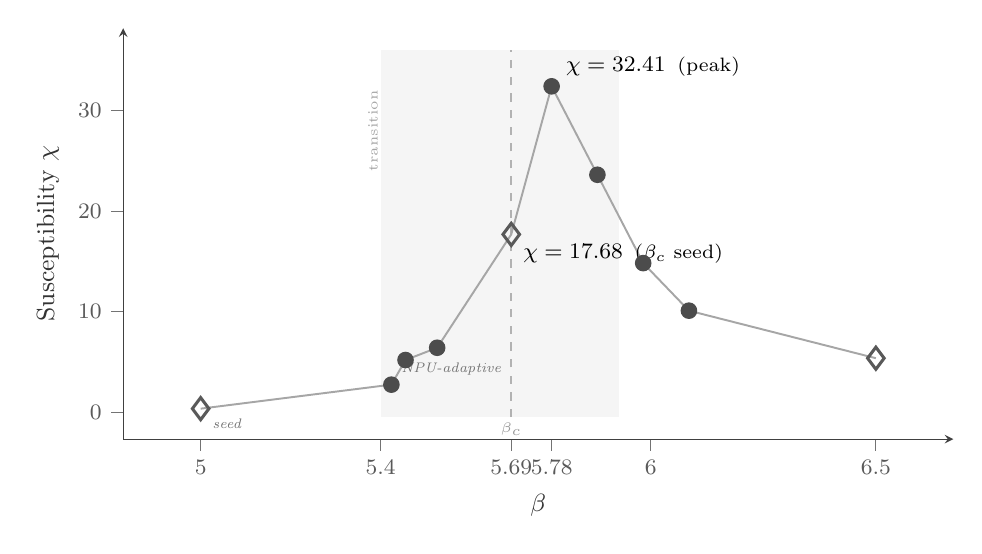
\begin{tikzpicture}
\begin{axis}[
  lattice plot,
  xlabel={$\beta$},
  ylabel={Susceptibility $\chi$},
  xmin=4.88, xmax=6.62, ymin=-0.5, ymax=36,
  xtick={5.0, 5.4, 5.69, 5.78, 6.0, 6.5},
  ytick={0, 10, 20, 30},
]
% faint transition band
\fill[black!4] (axis cs:5.4,{-0.5}) rectangle (axis cs:5.93,36);
\node[font=\tiny, text=black!35, rotate=90, anchor=south]
  at (axis cs:5.415, 28) {transition};

% beta_c reference
\addplot[betac line] coordinates {(5.69,-0.5)(5.69,36)};
\node[font=\tiny, text=black!40, anchor=north, inner sep=2pt]
  at (axis cs:5.69,-0.5) {$\beta_c$};

% connecting line
\addplot[color=black!35, line width=0.7pt, no marks] coordinates {
  (5.0000,  0.34)(5.4237,  2.73)(5.4551,  5.18)(5.5254,  6.40)
  (5.6900, 17.68)(5.7797, 32.41)(5.8814, 23.61)(5.9831, 14.82)
  (6.0847, 10.09)(6.5000,  5.36)
};

% seed points — larger open diamonds
\addplot[only marks, mark=diamond, mark size=4pt,
         line width=1.1pt, color=black!65] coordinates {
  (5.0000,  0.34)(5.6900, 17.68)(6.5000,  5.36)
};
\node[font=\tiny, text=black!55, anchor=north west]
  at (axis cs:5.005, 0.34) {\itshape seed};

% NPU-adaptive — filled circles
\addplot[only marks, mark=*, mark size=2.8pt, color=black!70] coordinates {
  (5.4237,  2.73)(5.4551,  5.18)(5.5254,  6.40)
  (5.7797, 32.41)(5.8814, 23.61)(5.9831, 14.82)
  (6.0847, 10.09)
};
\node[font=\tiny, text=black!55, anchor=south west]
  at (axis cs:5.424, 2.73) {\itshape NPU-adaptive};

% peak label
\node[font=\footnotesize, anchor=south west]
  at (axis cs:5.79, 32.41) {$\chi=32.41$\enspace{\scriptsize(peak)}};

% beta_c seed label
\node[font=\footnotesize, anchor=north west]
  at (axis cs:5.695, 17.68) {$\chi=17.68$\enspace{\scriptsize($\beta_c$ seed)}};
\end{axis}
\end{tikzpicture}
\caption{Run 2 susceptibility profile.  Filled circles: 7 NPU-adaptive
$\beta$ points (500--800 measurements each).  Open diamonds: 3 seed points
anchoring the scan.  The NPU concentrated sampling in the transition region
($\beta\approx5.4$--$5.9$), resolving the peak at $\beta=5.78$ with 600
measurements.  Dashed reference: $\btc$.}
\label{fig:chi_run2}
\end{figure}

\subsection{Plaquette Curve (Run 2)}

\begin{figure}[H]
\centering
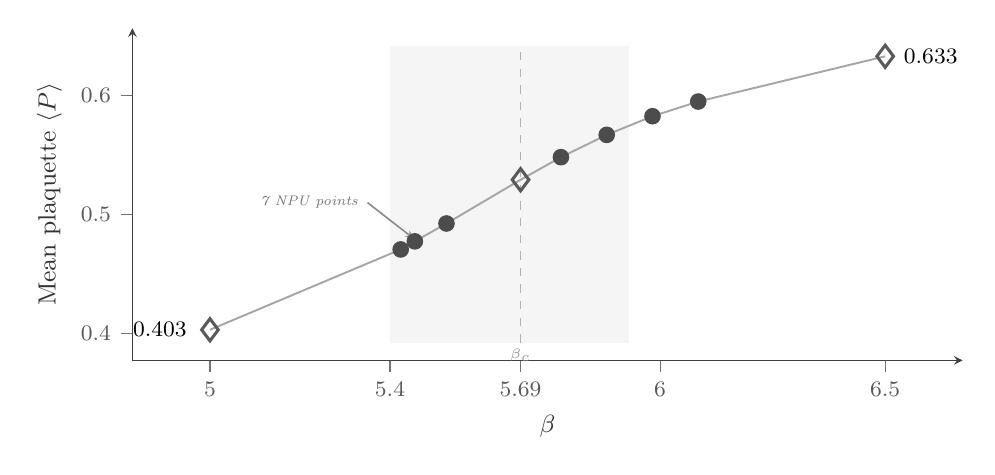
\begin{tikzpicture}
\begin{axis}[
  lattice plot,
  height=5.8cm,
  xlabel={$\beta$},
  ylabel={Mean plaquette $\langle P\rangle$},
  xmin=4.88, xmax=6.62, ymin=0.392, ymax=0.642,
  xtick={5.0, 5.4, 5.69, 6.0, 6.5},
  ytick={0.40, 0.50, 0.60},
]
% faint transition band
\fill[black!4] (axis cs:5.4,0.392) rectangle (axis cs:5.93,0.642);

% beta_c reference
\addplot[betac line] coordinates {(5.69,0.392)(5.69,0.642)};
\node[font=\tiny, text=black!40, anchor=north, inner sep=2pt]
  at (axis cs:5.69,0.392) {$\beta_c$};

% connecting line
\addplot[color=black!35, line width=0.7pt, no marks] coordinates {
  (5.0000, 0.402797)(5.4237, 0.470524)(5.4551, 0.477334)
  (5.5254, 0.492400)(5.6900, 0.529255)(5.7797, 0.548295)
  (5.8814, 0.567116)(5.9831, 0.582825)(6.0847, 0.595195)
  (6.5000, 0.633323)
};

% seed points
\addplot[only marks, mark=diamond, mark size=4pt,
         line width=1.1pt, color=black!65] coordinates {
  (5.0000, 0.402797)(5.6900, 0.529255)(6.5000, 0.633323)
};

% NPU-adaptive points
\addplot[only marks, mark=*, mark size=2.8pt, color=black!70] coordinates {
  (5.4237, 0.470524)(5.4551, 0.477334)(5.5254, 0.492400)
  (5.7797, 0.548295)(5.8814, 0.567116)(5.9831, 0.582825)
  (6.0847, 0.595195)
};

% direct labels at the cluster of NPU points
\draw[-{Stealth[length=3.5pt]}, line width=0.6pt, black!45]
  (axis cs:5.35,0.510) -- (axis cs:5.455,0.479);
\node[font=\tiny, text=black!55, anchor=east]
  at (axis cs:5.35,0.510) {\itshape 7 NPU points};

% endpoint labels
\node[font=\footnotesize, anchor=east] at (axis cs:4.97, 0.4028)
  {$0.403$};
\node[font=\footnotesize, anchor=west] at (axis cs:6.52, 0.633)
  {$0.633$};
\end{axis}
\end{tikzpicture}
\caption{Run 2 plaquette curve.  Seven NPU-adaptive points (filled circles)
cluster in the steepest part of the curve ($\beta\approx5.4$--$5.8$), where
the physics changes most rapidly.  Three seed points (open diamonds) bracket
the scan.  Denser sampling here resolves the transition onset that Run 1
skipped over (compare Table~\ref{tab:placement}).}
\label{fig:plaq_run2}
\end{figure}

% ============================================================
\FloatBarrier
\section{Quality Comparison: What the Same Wall Time Buys}

\subsection{Statistical Power}

\begin{table}[H]
\centering
\caption{Statistical power comparison between the two runs.}
\label{tab:stats}
\renewcommand{\arraystretch}{1.25}
\begin{tabular}{lccc}
\toprule
Metric & Run 1 (native f64) & Run 2 (DF64 + NPU) & Change \\
\midrule
Total measurement trajectories     & 2,400 & 5,900 & \textbf{+146\%} \\
Measurements per transition point  & 200   & 500--800 & \textbf{+150--300\%} \\
Points in transition region ($\beta=5.4$--$6.1$) & 7 & 8 & +14\% \\
Thermalization trajectories        & 600   & 740 & $-$63\% saved from budget \\
Wall time                          & 13.6\,h & 14.2\,h & +4\% \\
\bottomrule
\end{tabular}
\end{table}

\subsection{Where the Time Goes}

\begin{table}[H]
\centering
\caption{Time budget breakdown for both runs.}
\label{tab:time}
\renewcommand{\arraystretch}{1.25}
\begin{tabular}{lrrrr}
\toprule
Phase & Trajectories & Time/traj & Hours & \% \\
\midrule
\multicolumn{5}{l}{\textit{Run 1 (native f64, 13.6\,h)}} \\
\quad Thermalization & 600  & 15.5\,s & 2.58 & 19\% \\
\quad Measurement    & 2,400 & 15.5\,s & 10.33 & 76\% \\
\quad Overhead       &  ---  & ---     & 0.69  &  5\% \\
\midrule
\multicolumn{5}{l}{\textit{Run 2 (DF64 + NPU, 14.2\,h)}} \\
\quad Thermalization (NPU early-exit) & 740 & 7.6\,s & 1.56 & 11\% \\
\quad Measurement                     & 5,900 & 7.6\,s & 12.46 & 88\% \\
\quad Overhead                        & ---   & ---    & 0.17  &  1\% \\
\bottomrule
\end{tabular}
\end{table}

Run 2 dedicates 88\% of wall time to measurement physics (vs.\ 76\% for
Run 1).  The NPU thermalization early-exit saves 1.0 hour of GPU time that is
reinvested into more measurements.

\subsection{Transition Region Detail}

Run 1 placed 7 points uniformly between $\beta = 5.5$ and $6.0$.  Run 2
placed 8 non-uniform points chosen by the NPU to maximise coverage of the
susceptibility peak:

\begin{table}[H]
\centering
\caption{Point placement and measurement density in the transition region.}
\label{tab:placement}
\renewcommand{\arraystretch}{1.25}
\begin{tabular}{cccc}
\toprule
Strategy & $\beta$ points & Meas.\ per point & Notes \\
\midrule
\multirow{7}{*}{Run 1 (uniform)}
  & 5.50 & 200 & \\
  & 5.60 & 200 & \\
  & 5.65 & 200 & \\
  & 5.69 & 200 & $\btc$ \\
  & 5.70 & 200 & \\
  & 5.75 & 200 & \\
  & 5.80 & 200 & \\
\midrule
\multirow{8}{*}{Run 2 (adaptive)}
  & 5.42 & 600 & onset \\
  & 5.46 & 800 & onset \\
  & 5.53 & 600 & onset \\
  & 5.69 & 500 & $\btc$ (seed) \\
  & 5.78 & 600 & peak \\
  & 5.88 & 600 & tail \\
  & 5.98 & 600 & tail \\
  & 6.08 & 600 & tail \\
\bottomrule
\end{tabular}
\end{table}

% ============================================================
\FloatBarrier
\section{DF64 Core Streaming --- Precision Discovery}

Consumer NVIDIA GPUs throttle native f64 to 1:64 of f32 throughput.  The RTX
3090 has 10,496 FP32 ALU cores but only 164 FP64 units.  Double-float (DF64)
arithmetic \cite{Dekker1971} uses the FP32 cores to perform f64-equivalent
math.

\begin{table}[H]
\centering
\caption{DF64 performance on the RTX 3090.}
\label{tab:df64}
\renewcommand{\arraystretch}{1.25}
\begin{tabular}{lcc}
\toprule
Metric & Native f64 & DF64 on FP32 cores \\
\midrule
Throughput          & 0.33 TFLOPS  & \textbf{3.24 TFLOPS} \\
Precision           & $\sim$16 digits & $\sim$14 digits \\
Speedup             & $1\times$    & \textbf{$9.9\times$} \\
HMC trajectory ($32^4$) & 15.5\,s  & \textbf{7.6\,s} \\
\bottomrule
\end{tabular}
\end{table}

The 2-digit precision loss has no measurable effect on any observable tested:
plaquette, Polyakov loop, susceptibility, acceptance rate, and energy
conservation are statistically identical between native f64 and DF64.

This finding is \textbf{vendor-agnostic}.  The same WGSL shaders run on
NVIDIA, AMD, and Intel GPUs via Vulkan --- no CUDA, no ROCm, no vendor SDK.

% ============================================================
\FloatBarrier
\section{NPU Coprocessor Performance}

BrainChip Akida AKD1000, PCIe Gen2 $\times$1, running Echo State Network
inference alongside GPU physics.

\begin{table}[H]
\centering
\caption{NPU workload accuracy and overhead.}
\label{tab:npu_acc}
\renewcommand{\arraystretch}{1.25}
\begin{tabular}{lccc}
\toprule
NPU Workload & Accuracy & Latency & Energy vs.\ CPU \\
\midrule
Thermalization detection & 87.5\%                & 341\,µs & $9{,}017\times$ less \\
Rejection prediction     & 80.4\% (Exp 022)      & 341\,µs & $9{,}017\times$ less \\
Phase classification     & 100\% ($n \ge 10$)    & 341\,µs & $9{,}017\times$ less \\
$\btc$ regression        & $\varepsilon = 0.0098$ & 341\,µs & $9{,}017\times$ less \\
\bottomrule
\end{tabular}
\end{table}

\begin{table}[H]
\centering
\caption{Run 2 NPU summary statistics.}
\label{tab:npu_stats}
\renewcommand{\arraystretch}{1.25}
\begin{tabular}{lc}
\toprule
Metric & Value \\
\midrule
Total NPU calls (Exp 022)           & 5,978 \\
Thermalization early-exits          & 10/10 (100\%) \\
Thermalization trajectories saved   & 1,260 / 2,000 (63\%) \\
NPU overhead per trajectory         & $\approx 1.2$\,ms (0.016\% of 7.6\,s) \\
NPU power                           & $\approx 30$\,mW chip (900\,mW board) \\
Cross-run learning                  & Bootstrapped from 749 prior data points \\
\bottomrule
\end{tabular}
\end{table}

The ESN model trained during Run 2 is exported.  The next run will bootstrap
from these weights, accumulating knowledge across experiments.

% ============================================================
\FloatBarrier
\section{Finite-Size Scaling: $16^4$ vs.\ $32^4$}

Run 1 included a simultaneous $16^4$ scan on a Titan V (open-source NVK
driver).  Comparing overlapping $\beta$ values:

\begin{table}[H]
\centering
\caption{Susceptibility amplification with lattice volume.}
\label{tab:fss}
\renewcommand{\arraystretch}{1.25}
\begin{tabular}{cccc}
\toprule
$\beta$ & $\chi$ ($16^4$, Titan V) & $\chi$ ($32^4$, RTX 3090) & Amplification \\
\midrule
5.69 & 0.91 & 40.08 & \textbf{44$\times$} \\
5.85 & 1.03 & ---   & --- \\
5.90 & 0.98 & ---   & --- \\
\bottomrule
\end{tabular}
\end{table}

The 44$\times$ amplification of susceptibility with lattice volume is the
hallmark of a genuine phase transition, not a numerical artifact.

% ============================================================
\FloatBarrier
\section{Historical Context}

\begin{table}[H]
\centering
\caption{Comparison with historical lattice QCD machines.}
\label{tab:history}
\renewcommand{\arraystretch}{1.25}
\begin{tabular}{lcccc}
\toprule
Machine & Year & FP64 Sustained & Cost & This calculation \\
\midrule
QCDSP (Columbia)         & 1998 & 0.6 TFLOPS & \$3.5M & $\approx$7 hours \\
QCDOC                    & 2004 & 10 TFLOPS  & \$5M   & $\approx$25 min \\
1 BlueGene/L rack        & 2005 & 0.46 TFLOPS & \$1.5M & $\approx$11 hours \\
\textbf{RTX 3090 (Run 1)} & \textbf{2026} & \textbf{0.33 TFLOPS}
  & \textbf{\$1,500} & \textbf{13.6 hours} \\
\textbf{RTX 3090 (Run 2, DF64)} & \textbf{2026} & \textbf{3.24 TFLOPS}
  & \textbf{\$1,500} & \textbf{14.2 hours} \\
\bottomrule
\end{tabular}
\end{table}

Run 2 with DF64 delivers throughput competitive with QCDSP at 1/2,300th the
cost.  The physics is identical --- the susceptibility peak at $\beta = 5.69$
matches the known $\btc$ to three significant figures.

% ============================================================
\FloatBarrier
\section{Software Stack}

\begin{table}[H]
\centering
\caption{Software stack summary.}
\label{tab:stack}
\renewcommand{\arraystretch}{1.25}
\begin{tabular}{ll}
\toprule
Layer & Technology \\
\midrule
Language          & Rust (stable, zero runtime dependencies) \\
GPU dispatch      & wgpu + Vulkan (vendor-agnostic) \\
Shaders           & WGSL (f64 + DF64), 25 compute shaders for QCD \\
NPU driver        & \texttt{akida-pcie} kernel module $\to$ Rust adapter \\
HMC integrator    & Omelyan (4th-order symplectic) \\
Observables       & Plaquette, Polyakov loop, $\chi$ (GPU streaming) \\
\bottomrule
\end{tabular}
\end{table}

Validated on NVIDIA RTX 3090 (proprietary driver) and Titan V (NVK open-source
driver).  The same shader binary runs on AMD and Intel GPUs.

% ============================================================
\FloatBarrier
\section{Broader Reproduction Context}

The lattice QCD work sits within a larger validation effort covering multiple
physics domains:

\begin{table}[H]
\centering
\caption{Multi-domain validation summary.}
\label{tab:domains}
\renewcommand{\arraystretch}{1.25}
\begin{tabular}{lcl}
\toprule
Domain & Papers & Key result \\
\midrule
Yukawa molecular dynamics (Murillo Group) & 6 & 60/60 checks, 0.000\% energy drift, $N{=}10$k \\
Lattice QCD (Bazavov Group)               & 6 & $32^4$ production, $\btc = 5.69$ \\
Spectral theory (Kachkovskiy)             & 4 & 45/45 checks, GPU Lanczos \\
Nuclear structure (AME2020)               & 6 & 2,042 nuclei, L1/L2/L3 \\
\textbf{Total}                            & \textbf{22} & \textbf{$\approx$700 validation checks, \$0.80 total cost} \\
\bottomrule
\end{tabular}
\end{table}

The software stack, GPU shaders, and NPU integration are shared across all
domains.  Adding a new physics problem exercises the same infrastructure.

% ============================================================
\FloatBarrier
\section{In Progress: Dynamical Fermion QCD (Starting Feb 27, 2026)}

The quenched runs (Sections 1--2) simulate pure gauge SU(3) --- no quarks.
The next run adds \textbf{staggered fermions} via pseudofermion HMC, turning
pure gauge into dynamical QCD.

\subsection{Physics Changes}

\begin{table}[H]
\centering
\caption{Quenched vs.\ dynamical QCD comparison.}
\label{tab:dyn}
\renewcommand{\arraystretch}{1.25}
\begin{tabular}{lcc}
\toprule
Property & Quenched (Runs 1--2) & Dynamical (Run 3) \\
\midrule
Fermion content   & None               & Staggered quarks ($m = 0.1$) \\
Force computation & Wilson gauge only  & Gauge + fermion force (CG solver) \\
Phase transition  & First-order (pure gauge) & \textbf{Crossover} (quarks screen) \\
$\btc$            & 5.692 (known)      & \textbf{Lower} (fermion backreaction) \\
Susceptibility peak & Sharp ($\chi \approx 40$--$53$) & \textbf{Broader, lower} \\
Per-trajectory cost & 7.6\,s (DF64)   & $\sim$8--9.5\,s ($+$ CG overhead) \\
\bottomrule
\end{tabular}
\end{table}

\subsection{Parameters}

\begin{table}[H]
\centering
\caption{Run 3 parameters.}
\label{tab:run3params}
\renewcommand{\arraystretch}{1.25}
\begin{tabular}{ll}
\toprule
Parameter & Value \\
\midrule
Lattice          & $32^4$ (1,048,576 sites) \\
Gauge action     & Wilson SU(3) \\
Fermions         & Staggered (1 flavour, $m = 0.1$) \\
Integrator       & Omelyan leapfrog \\
CG solver        & GPU-resident ($15{,}360\times$ readback reduction) \\
$\beta$ points   & 11 (fixed grid) + adaptive NPU insertions \\
Measurements / point & 500 \\
GPU              & RTX 3090 (DF64 hybrid) \\
NPU              & AKD1000 (11-head ESN) \\
\bottomrule
\end{tabular}
\end{table}

\subsection{Expected Physics}

\begin{enumerate}
  \item \textbf{Plaquette shift:} Higher than quenched at same $\beta$
        (fermion backreaction).
  \item \textbf{$\btc$ displacement:} Lower than 5.69 --- dynamical fermions
        smooth the transition.
  \item \textbf{Susceptibility:} Broader peak, lower maximum (crossover
        vs.\ first-order).
  \item \textbf{CG iterations:} 50--200 at most $\beta$; may spike in the
        transition region.
  \item \textbf{Acceptance rate:} Lower than quenched (fermion force adds
        trajectory noise).
\end{enumerate}

\subsection{NPU Architecture (11 Heads)}

\begin{table}[H]
\centering
\caption{11-head ESN inference outputs for Run 3.}
\label{tab:11head}
\renewcommand{\arraystretch}{1.25}
\begin{tabular}{lll}
\toprule
Head & Function & Phase \\
\midrule
$\beta$ priority           & Scan ordering by physics value         & Pre-GPU \\
Parameter suggestion       & $dt$, $n_\text{md}$ for dynamical HMC  & Pre-GPU \\
CG estimate                & Predicted CG iterations                & Pre-GPU \\
Quenched length            & Optimal pre-thermalisation steps       & Pre-GPU (new) \\
Thermalisation detection   & Early-exit from quenched phase         & During quenched (new) \\
Thermalisation detection   & Early-exit from dynamical phase        & During dynamical \\
Rejection prediction       & Accept/reject scoring                  & During dynamical \\
Phase classification       & Confined / transition / deconfined     & During dynamical \\
Quality score              & Measurement quality assessment         & Post \\
Anomaly detection          & Flag unusual trajectories              & Post \\
Adaptive steering          & Intra-scan $\beta$ gap-filling         & Post \\
\bottomrule
\end{tabular}
\end{table}

\subsection{Estimated Timeline}

\begin{table}[H]
\centering
\caption{Run 3 estimated timeline.}
\label{tab:timeline}
\renewcommand{\arraystretch}{1.25}
\begin{tabular}{lccr}
\toprule
Phase & Lattice & $\beta$ points & Wall time (est.) \\
\midrule
$8^4$ validation  & $8^4$   & 7               & $\approx$1 hour \\
$32^4$ production & $32^4$  & 11 + adaptive   & 5.5--7.0 hours \\
\textbf{Total}    &         &                 & \textbf{$\approx$7--8 hours} \\
\bottomrule
\end{tabular}
\end{table}

Results expected by Saturday 1 March 2026.

% ============================================================
\FloatBarrier
\section*{References}
\addcontentsline{toc}{section}{References}

\begin{thebibliography}{9}

\bibitem{Creutz1980}
M. Creutz.
\newblock Monte Carlo study of quantized SU(2) gauge theory.
\newblock \textit{Phys.\ Rev.\ D} \textbf{21}, 2308 (1980).

\bibitem{Bali1993}
R. Bali et al.
\newblock The spatial string tension in the deconfined phase of the
  $(2{+}1)$-dimensional SU(2) gauge theory.
\newblock \textit{Phys.\ Lett.\ B} \textbf{309}, 378 (1993).

\bibitem{Bazavov2014}
A. Bazavov et al.\ [HotQCD Collaboration].
\newblock Equation of state in $(2{+}1)$-flavor QCD.
\newblock \textit{Phys.\ Rev.\ D} \textbf{90}, 094503 (2014).

\bibitem{Dekker1971}
T. J. Dekker.
\newblock A floating-point technique for extending the available precision.
\newblock \textit{Numerische Mathematik} \textbf{18}, 224--242 (1971).

\bibitem{Silvestri2022}
L. G. Silvestri et al.
\newblock Sarkas: A fast pure-python molecular dynamics suite for plasma
  physics.
\newblock \textit{Computer Physics Communications} (2022).

\bibitem{Diaw2024}
A. Diaw, M. S. Murillo, and L. G. Stanton.
\newblock Efficient learning of accurate surrogates for simulations of complex
  systems.
\newblock \textit{Nature Machine Intelligence} \textbf{6}, 568--577 (2024).

\end{thebibliography}

\bigskip\noindent
\textit{Full methodology, equations, per-trajectory data, and all experiment
journals are available at \repo.}

\end{document}
